% !TEX root = seminararbeit.tex

\section{Basics and Related Work}
\label{basics-and-related-work}

\subsection{Scene-Graph}\label{scene-graph}

Scene-graphs can be used to group and organize 3D objects, their
properties and concerning transformations. A directed acyclic graph
(DAG) can be used to represent a scene-graph. It starts with a root node
that is associated with one or more children. Each child can be an
object or a group, again containing more children. A group can contain
associated transformation information, like \emph{translation},
\emph{rotation} or \emph{scaling}. This structure has certain advantages
compared to applying all transformations to the raw meshes and sending
everything to the \gls{GPU}. \cite{realityprime}

\hyperref[ssiml]{SSIML} scene-graphs differ from the above definition:
there are three types of nodes:
\begin{itemize*}
  \item transform
  \item geometry
  \item group
\end{itemize*}

\subsubsection{Culling}\label{culling}

Before using structures like scene-graphs, all polygon would be sent to
the \gls{GPU} and the \gls{GPU} would need to test what polygons are actually in the
view and thus need to be rendered. The problem with that approach was
that this information was only known after doing a lot of calculations
for every polygon already.\\
With a scene-graph it's possible to start from the root and traverse the
graph, testing the bounding box of each group and only sending it to the
\gls{GPU} it it's completely visible. If it ain't, the whole sub-tree isn't
sent to the \gls{GPU}. If it's partially visible the same process is applied
to the sub-tree.\\
By using a structure that retains more information about what it
represents it's possible to let the CPU do more of the heavy
lifting and unburden the \gls{GPU}.

\begin{quote}
  Rather than do the heavy work at the OpenGL and polygon level,
  scene-graph architects realized they could better perform culling at
  higher level abstractions for greater efficiency. If we can remove the
  invisible objects first, then we make the hardware do less work and
  generally improve performance and the all-important frame-rate. \cite{realityprime}
\end{quote}

\subsubsection{Transformations}\label{transformations}

Another advantage is the way transformations work. Instead of applying
them to the meshes directly, and keeping track of what meshes belong to
the same object (like the chassis and the tires and the windows of a
car), they can simply be nested under the same transformation group. The
transformation thus applies to all objects associated with that group.

\subsubsection{Reuse}\label{reuse}

With the ability to address nodes it's possible to reuse their
information. If you have a car, it would be enough to have only one node
containing the geometry for a tire, all other tires are merely addressing
the tire with the geometry information (see listing \ref{list:defuse}).
That way the memory footprint of an application can be reduced.

\begin{figure}
  \begin{minted}{html}
<Group>
  <Transform>
    <Shape def="chassis">
        <Appearance>
            <Material></Material>
        </Appearance>
        <Box></Box>
    </Shape>
  </Transform>
  <Transform>
    <Shape def="tire">
        <Appearance>
             <Material></Material>
        </Appearance>
        <Torus></Torus>
    </Shape>
  </Transform>
  <Transform>
    <Shape use="tire"/>
  </Transform>
  <Transform>
    <Shape use="tire"/>
  </Transform>
  <Transform>
    <Shape use="tire"/>
  </Transform>
</Group>
  \end{minted}
  \caption{example x3d group showing the use of \texttt{def} and \texttt{use}}
  \label{list:defuse}
\end{figure}


\subsubsection{X3D}\label{x3d}

X3D is the XML representation of VRML which was designed as
a universal interactive 3D exchange format, much like html is for
written documents or \gls{SVG} for vector graphics. Due to its XML structure
it can be integrated in html documents, thus the Frauenhofer Institute
pursued to implement a runtime that could interpret and visualize X3D in
the browser, by using a WebGL context. It's called
\href{http://www.x3dom.org/}{x3dom} and it's extensively used by
SceGraToo, the tool that arose from this thesis.

\paragraph{x3dom}
\label{par:x3dom}

As said in the previous chapter x3dom was developed by the Frauenhofer
Institute to realize the vision that started VRML in the first place:
\emph{mark up interactive 3D content for the web}. On the web there are
to entirely different approaches to describe the same thing:
\begin{itemize*}
  \item imperative
  \item declarative
\end{itemize*}

The matrix in table \ref{tab:feature_matrix} classifies x3dom together with other common web
technologies \cite{x3dom}:

\begin{table}[H]
  \begin{longtable}[c]{@{}lll@{}}
  \toprule
  & 2D & 3D\tabularnewline
  \midrule
  \endhead
  Declarative & \gls{SVG} \cite{svg} & x3dom \cite{x3dom} \tabularnewline
  Imperative  & Canvas \cite{canvas} & WebGL \cite{webgl} \tabularnewline
  \bottomrule
  \end{longtable}
  \caption{\cite{x3dom}}
  \label{tab:feature_matrix}
\end{table}

As can be seen in table \ref{tab:feature_matrix} x3dom complements the already existing technologies
perfectly.

\subsection{SSIML}
\label{ssiml}

Heterogeneous developer groups, groups that are comprised of people from
different backgrounds (programmers, 3D designers) have hard time working
together. \cite{Glinz:2015:SUS:2802768.2802838}

SSIML is a graphical approach to unify the scene-graph model and the the
application model, thus making the communication between the different
parties easier.

It also serves as a code generation template.

\begin{figure}[htbp]
  \centering
  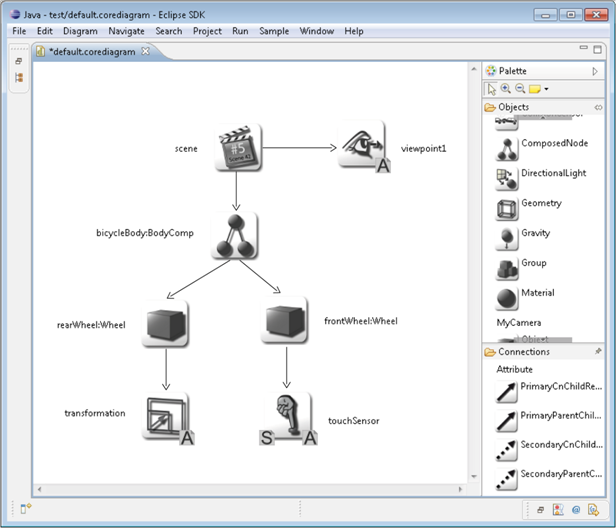
\includegraphics[width=12cm]{../assets/SSIML.png}
	\caption{A SSIML Diagram \cite{roundtrip3dwebsite}}
	\label{fig:ssimldiagram}
\end{figure}

\subsection{Roundtrip 3D}\label{roundtrip-3d}

As stated above, when developing 3D applications, many different
developers are involved, i.e.~3D designers, programmers and, ideally,
also software designers (see figure \ref{fig:ssimldiagram})

% TODO: convert to pdf
% 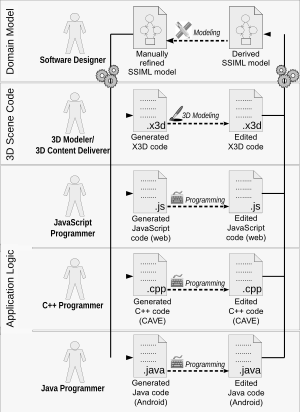
\includegraphics{../assets/csrd2014.svg}\\
% Roundtrip3D proposed process
% \href{http://dx.doi.org/10.1007/s00450-014-0258-8}{JLV15}

Roundtrip3D was research project that, amongst others, resulted in a
graphical editor for \hyperref[ssiml]{SSIML} models. It offers an
approach for merging a developer's changes back into the main model.
After all working copies are merged back into the main model (dropping
unwanted or conflicting changes), all working copies are regenerated and
delivered to the individual developers. After each roundtrip every
developer has a copy of the project that is consistent with everyone
else's.

\subsubsection{states}\label{states}

TODO:
\begin{itemize}
  \item explaing the DOM
  \item move to implemtation
\end{itemize}

Using something imperative like backbone it would be necessary to create
a model (copying the information already in the DOM), a view (rendering
that information to the DOM again) and a controller keeping track of the
state changing the model where necessary and rerendering the view, and
also keeping track of all it's children and removing them when they
disappear or creating new ones whenever a new X3D element appears.

\subsubsection{Functional Programming}\label{functional-programming}

All SceGraToo does is listen to changes of the \gls{X3D} node and whenever it
changes, may it be an attribute that changes or nodes that are added or
removed, it calls one function that evaluates the X3D node (basically
traversing it) and return the new structure. That structure is diffed
against the tree-view that is already in the DOM and react calculates
the minimal changes necessary to make the tree-view's old structure
coherent with the newly calculated one.

\subsection{Koa}\label{koa}

TODO: move to implemenation Koa is pretty much boring unless I'd explain
node.js's take on asynchronicity, callbacks, promises and then
generators. Still, the server is way to simple to be of any interest for
this project.

\subsection{Related Work}
\label{related-work}

\subsubsection{Collaborative Work}
\label{collaborative-work}
 
\subsubsection{\texorpdfstring{\href{http://3d.meteor.com/}{3D
Meteor}}{3D Meteor}}\label{d-meteor0}

\begin{figure}[htbp]
  \centering
  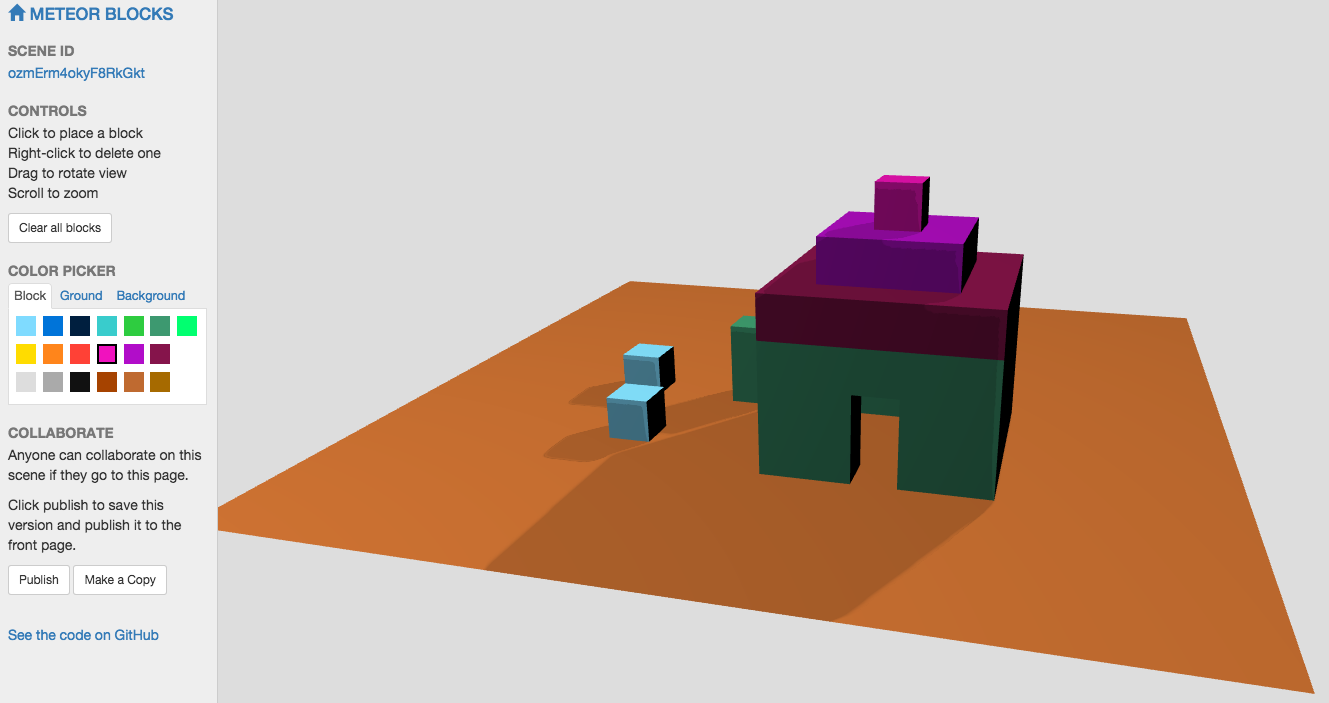
\includegraphics[width=12cm]{../assets/3dmeteor.png}
  \caption{3D Meteor}
	\label{fig:3dmeteor}
\end{figure}

This simple 3D editor allows the user to add and remove colored blocks
to a scene. The synchronization is leveraging meteor's database
collection subscription features. Meteor apps are comprised of a client
side and a server side. The client can subscribe to database collections
and get's automatically notified of changes to that collection by the
server. The only thing that actually is synchronized is an array of
\emph{boxes}. A box is an object with an x, y and z property describing
its position.

\subsubsection{Blender Plugin}
\label{blender-plugin}

I don't do anything about collaborative working anymore. So yeah.

As part of an asset management system the Université du Québec à
Montréal implemented a plugin for blender for collaborative working. An
artist can record changes to to wiremeshes and store them on a server.
Another artist can download these changes and apply them to his working
copy. The diffs are a simple list of vertices and their movement in the
x, y and z space. \cite{LCR07}

\begin{verbatim}
95 [0.0000, 0.0000, 0.0000]
295 [0.0027, 0.0013, 0.0000]
309 [0.2123, 0.1001, 0.0000]
311 [0.3029, 0.1429, 0.0000]
\end{verbatim}

These are saved on the server and another user working on the same
object can apply them to his working copy. They can actually be applied
to any object that has the same number of vertices. That's also a
shortcoming. Adding or removing vertices cannot be handled by the
plugin. It is also not in real time, so it is more comparable to version
control system like git, just for 3d models.

\subsubsection{3D Widgets}\label{d-widgets}

\paragraph{\texorpdfstring{\href{http://www.tiltbrush.com/}{Tilt
Brush}}{Tilt Brush}}\label{tilt-brush20}

Tilt Brush was lauded for it's 3d interface.

\subsubsection{Gizmos}\label{gizmos}

Gizmos, also called manipulators, are handles or bounding boxes with
handles that manipulate it's containgin object in a predefined way when
dragged. \cite{wikigizmo}

In X3D gizmos can be realized with on of X3DDragSensorNode's \cite{x3ddragsensornode} decedents.

\begin{description*}
\item[SphereSensor]
  SphereSensor converts pointing device motion into a spherical rotation around the origin of the local coordinate system. \cite{spheresensor}
\item[CylinderSensor]
  The CylinderSensor node converts pointer motion (for example, from a mouse) into rotation values, using an invisible cylinder of infinite height, aligned with local Y-axis. \cite{cylindersensor}
\item[PlaneSensor]
  PlaneSensor converts pointing device motion into 2D translation, parallel to the local Z=0 plane. Hint: You can constrain translation output to one axis by setting the respective minPosition and maxPosition members to equal values for that axis.
  \cite{planesensor}
\end{description*}

The sensors track drag events on their siblings. In the example in figure \ref{fig:x3dgizmo}
(which is taken directly from the x3dom website) the PlaneSensor tracks
drag events on the cones and the cylinder that make up the cyan handle.

Every time it detects a drag event it converts it into a 2D
transformation and raises an \emph{onOutPutChange} event. The callback
\texttt{processTranslationGizmoEvent} is registered as an event handler.
In this function the position of the handle is adjusted to make it
follow the drag movement, also the position of the teapot is adjust.

Having the the handles being 3d objects within the scene, that look
touchable and intractable, make it easier for users find their way
around the application. Instead of haven to learn keyboard shortcuts the
user simply uses their intuition about how she would interact with
objects in the real world.

\begin{minted}[breaklines,bgcolor=bg]{html}
<group>
  <planeSensor autoOffset='true' axisRotation='1 0 0 -1.57' minPosition='-6 0' maxPosition='6 0' onoutputchange='processTranslationGizmoEvent(event)'>
  </planeSensor>

  <transform id='translationHandleTransform'>
    <transform translation='0 -5.5 8' rotation='0 1 0 1.57'>
      <transform translation='0 0 1.5' rotation='1 0 0 1.57'>
        <shape DEF='CONE_CAP'>
          <appearance DEF='CYAN_MAT'><material diffuseColor='0 1 1'></material></appearance>
          <cone height='1'></cone>
        </shape>
      </transform>
      <transform rotation='1 0 0 -1.57'>
        <shape>
          <appearance USE='CYAN_MAT'></appearance>
          <cylinder></cylinder>
        </shape>
      </transform>
      <transform translation='0 0 -1.5' rotation='1 0 0 -1.57'>
        <shape USE='CONE_CAP'></shape>
      </transform>
    </transform>
  </transform>
</group>
\end{minted}

\begin{figure}[htbp]
  \begin{minipage}{.5\textwidth}
    \centering
    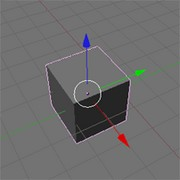
\includegraphics[width=0.9\textwidth]{../assets/Manual-Manipulators-Translate.jpg}
  	\caption{translation gizmo \cite{blenderwiki}}
  \end{minipage}
  \begin{minipage}{.5\textwidth}
    \centering
    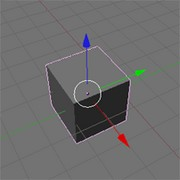
\includegraphics[width=0.9\textwidth]{../assets/Manual-Manipulators-Translate.jpg}\\
  	\caption{rotation gizmo \cite{blenderwiki}}
  \end{minipage}\\
  \begin{minipage}{.5\textwidth}
    \centering
    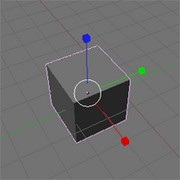
\includegraphics[width=0.9\textwidth]{../assets/Manual-Manipulators-Scale.jpg}
  	\caption{scale gizmo \cite{blenderwiki}}
  \end{minipage}
  \begin{minipage}{.5\textwidth}
    \centering
    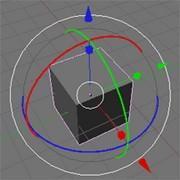
\includegraphics[width=0.9\textwidth]{../assets/Manual-Manipulators-Combo.jpg}
  	\caption{all gizmos together \cite{blenderwiki}}
  \end{minipage}
\end{figure}
\begin{figure}[]
  \centering
  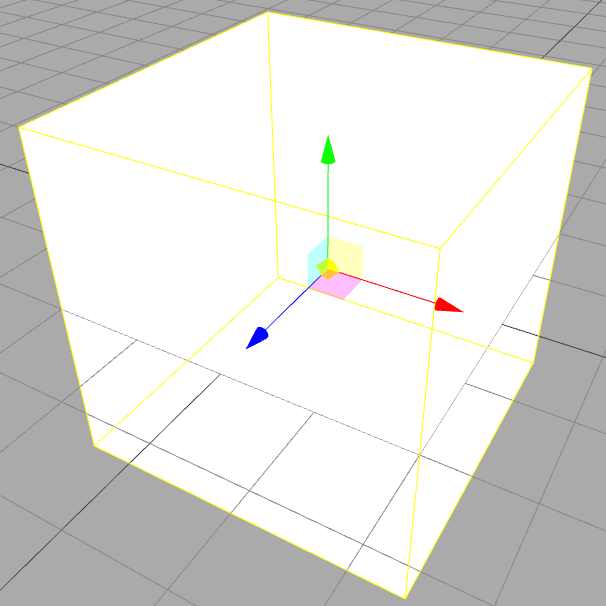
\includegraphics[width=12cm]{../assets/threejs-editor.png}
	\caption{ Shows translate gizmos along the x, y and z axis als well as gizmos that translate the cube along the xy, xz, yz and frustum plane. \cite{threejseditor} }
\end{figure}
\begin{figure}[]
  \centering
  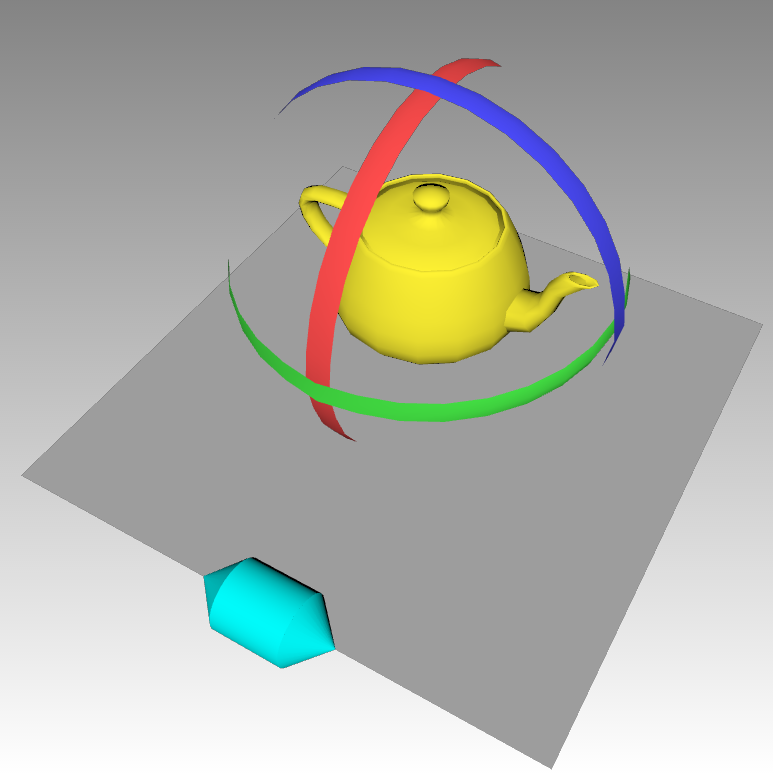
\includegraphics[width=12cm]{../assets/x3dom-gizmo-example.png}
	\caption{ Shows an official x3dom tutorial for using sensors to create gizmos. \cite{x3dgizmo} }
	\label{fig:x3dgizmo}
\end{figure}

\clearpage
\subsubsection{\texorpdfstring{\href{https://github.com/x3dom/component-editor}{Component
Editor}}{Component Editor}}\label{component-editor30}

\begin{itemize*}
\item release 12th of june 2015
\item thus after the work on SceGraToo started
\item developed over a year
\item developed by 3 people working part time
\item cannot save or load x3d files
\item serealizes the scene into a JSON format
\end{itemize*}

\begin{minted}[breaklines,bgcolor=bg]{json}
{
  "0": {
    "type": "Box",
    "transform": "1.000000, 0.000000, 0.000000, 0.000000, \n0.000000, 1.000000, 0.000000, 0.000000, \n0.000000, 0.000000, 1.000000, 0.000000, \n0.000000, 0.000000, 0.000000, 1.000000",
    "referencePoints": ["p1", "p2", "p3", "p4", "p5", "p6"],
    "parameters": {
      "Size": [1, 1, 1],
      "Positive Element": "true"
    }
  }
}
\end{minted}

\begin{itemize*}
\item
  this would loose meta information like the IDs in comments.
\end{itemize*}

\subsubsection{Real-Time Collaborative Scientific WebGL
Visualization with Web Sockets}
\label{rtcswvwws}

Using web sockets instead of AJAX is an interesting approach. \cite{Marion:2012:RCS:2338714.2338721} Especially
the cut down on latency. It is over all very similar to the approach I
was thinking about. Except that they propagate only some information,
like the camera position and view angle. In SceGraToo's case the whole
scene needs to be synchronized. So to have specttors like they have we
either have to send the whoe model to the server after eacht change or
use some kind of tree diff algorithm. They visualize a specific dataset
in a threejs's specific JSON format \cite{threejs-format}. We only need to visualize X3D
data, so there is no reason to use some generic Visualization tool kit,
x3dom does a pretty good job doint this. on the other hand we not only
have to visualize the data, but also manipulate it and this is way
easiear in a descriptive scene graph instead of manimpulatiing webgl
scenes or data formats like vtk.

\subsubsection{\texorpdfstring{ParaViewWeb
\href{http://paraviewweb.kitware.com/}{pvweb}}{ParaViewWeb pvweb}}\label{paraviewweb-pvweb}

Simple to use out of the box, but needs a paraview server instance and
paraview does not support x3d as an input format. So using this is sadly
not possible unless an import filter is written. The visualization is
mainly meant to explore data sets. There is no easy way to manipulate
the input data. This can only happen by extending the visualization
pipeline via python scripts on the server.
